\documentclass[dvipdfmx, 10pt]{jsarticle}
\usepackage{mathtools}
\usepackage[margin=20truemm]{geometry}
\usepackage{amssymb}
\usepackage{amsmath}
\usepackage{algorithm}
\usepackage{algpseudocode}
\usepackage{hyperref}
\usepackage{framed}

\title{\textbf{ニューラルネットワーク (Neural Network)}}
\author{}
\date{}

\begin{document}

\maketitle

\section*{基本構造}
\begin{itemize}
    \item \textbf{入力層 (Input Layer)}: 特徴量を受け取る層
    \item \textbf{隠れ層 (Hidden Layer)}: データを変換し, 特徴を抽出する層
    \item \textbf{出力層 (Output Layer)}: モデルの最終的な予測値を出力する層
    \item \textbf{ユニット (unit)}: 各ノードのこと. 入力を重み付き和で計算し, 活性化関数を適用する
\end{itemize}

\section*{ユニットが1つの場合}
1つのユニットにおける出力は以下のように計算される: 
\begin{align*}
    u &= \sum_{i=1}^n w_i x_i + b \\
    z &= f(u)
\end{align*}

\begin{itemize}
    \item $w_i$: 各入力に対する重み
    \item $x_i$: 各入力データ
    \item $b$: バイアス
    \item $u$: ユニット入力
    \item $z$: ユニット出力
    \item $f(u)$: 活性化関数
\end{itemize}

\section*{ユニットが複数の場合}
多層ニューラルネットワークについては以下のように計算される: 
\begin{align*}
    \mathbf{u}^{(\ell)} &= \mathbf{W}^{(\ell-1)} \mathbf{z}^{(\ell-1)} + \mathbf{b}^{(\ell-1)} \\
    \mathbf{z}^{(\ell)} &= f_{\ell}(\mathbf{u}^{(\ell)})
\end{align*}

\begin{itemize}
    \item $\mathbf{W}^{(\ell)}$: $\ell$層のパラメータ行列
    \item $\mathbf{b}^{(\ell)}$: $\ell$層のバイアス
    \item $\mathbf{u}^{(\ell)}$: $\ell$層へのユニット入力
    \item $\mathbf{z}^{(\ell)}$: $\ell$層からのユニット出力
    \item $f_{\ell}$: $\ell$層における活性化関数
\end{itemize}

\section*{ニューラルネットワークのイメージ}
\begin{figure}[H]
    \centering
    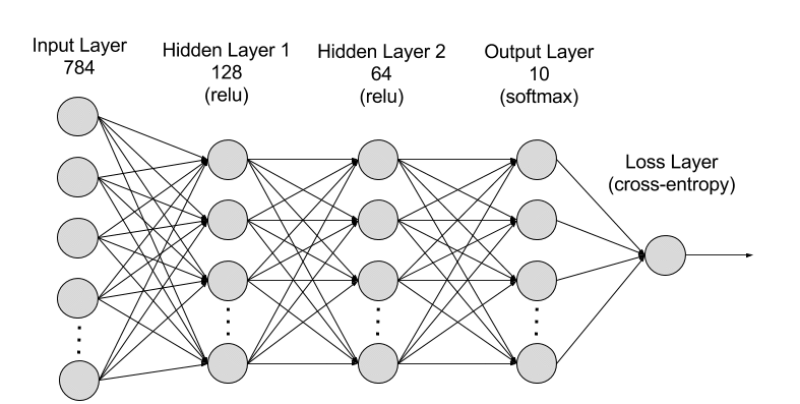
\includegraphics[width=0.5\textwidth]{NN_example.png}
    \caption{ニューラルネットワークのイメージ}
\end{figure}

\section*{順伝播}
\begin{enumerate}
    \item 入力データが層を通過し, 重み (Weights) とバイアス (Bias) を使用して計算する. 
    \item 各ノードで活性化関数 (Activation Function) を適用して非線形な結果を生成する. 
    \item 最後に出力層で結果を得る. 
\end{enumerate}

\section*{活性化関数}
\subsection*{恒等写像}
回帰の出力層に用いる. 
\begin{align*}
    u &= \sum_{i=1}^n w_i x_i + b \\
    f(u) &= u
\end{align*}
\begin{itemize}
    \item $w_i$: 各入力に対する重み
    \item $x_i$: 各入力データ
    \item $b$: バイアス
    \item $u$: ユニット入力
    \item $f(u)$: 活性化関数
\end{itemize}

\subsection*{ロジスティック (シグモイド) 関数}
2値分類の出力層に用いる. 
\begin{align*}
    u &= \sum_{i=1}^n w_i x_i + b \\
    f(u) &= \frac{1}{1 + \exp(-u)}
\end{align*}
\begin{itemize}
    \item $w_i$: 各入力に対する重み
    \item $x_i$: 各入力データ
    \item $b$: バイアス
    \item $u$: ユニット入力
    \item $f(u)$: 活性化関数
\end{itemize}

以下の性質を持つ: 
\begin{itemize}
    \item $\forall u \in \mathbb{R}, 0 < f(u) < 1$
    \item $\lim_{u\to \infty} f(u) = 1$
    \item $\lim_{u\to -\infty} f(u) = 0$
    \item $f(0) = 0.5$
\end{itemize}

\subsection*{softmax関数}
多クラス分類の出力層に用いる. 
\begin{align*}
    \mathbf{u} &= \mathbf{W} \mathbf{x} + \mathbf{b} \\
    f_k(\mathbf{u}) &= \frac{\exp(u_k)}{\sum^{K}_{\ell=1} \exp(u_{\ell})}
\end{align*}
\begin{itemize}
    \item $\mathbf{x}$: 入力
    \item $\mathbf{W}$: パラメータ行列
    \item $\mathbf{b}$: バイアス
    \item $\mathbf{u}$: ユニット入力
    \item $f_k$: ベクトルのk番目に対応する活性化関数
\end{itemize}

以下の性質を持つ: 
\begin{itemize}
    \item $\forall u \in \mathbb{R}, 0 < f_k(\mathbf{u}) < 1$
    \item $\sum^{K}_{k=1} f_k(\mathbf{u}) = 1$
    \item $K=2$のとき, シグモイド関数と一致する
\end{itemize}

$K = 2$の場合, 2つのクラスに対応する出力$u_1, u_2$に対して: 
\begin{align*}
    f_1 &= \frac{\exp(u_1)}{\exp(u_1) + \exp(u_2)} = \frac{1}{1 + \exp(-(u_1 - u_2))}
\end{align*}
これはシグモイド関数の形と一致する. 

\section*{多層NNにおける学習}
\begin{itemize}
    \item 既知事例 $\{(x_{(1)}, y_{(1)}), (x_{(2)}, y_{(2)}), \ldots, (x_{(N)}, y_{(N)})\}$
    \item 既知事例のラベル $y_n$ とモデル出力 $z^{(L)}$ に対して, 損失関数 $L(W)$ を最小化するように各層のパラメータ $W^{(\ell)}$ を学習
\end{itemize}

\section*{損失関数}
\subsection*{回帰}
二乗誤差を最小にするので: 
\begin{align*}
    L(W) = \frac{1}{N} \sum_{n=1}^N \| y_{(n)} - z^{(L)}_{(n)} \|_2^2
\end{align*}

\subsection*{二値分類}
$y=1$となる最大尤度を求めるので: 
\begin{align*}
    L(W) = \sum_{n=1}^N \log(1 + \exp(-y_{(n)} z^{(L)}_{(n)}))
\end{align*}

\subsection*{多クラス分類}
各ラベルが1の時の最大尤度を求めるので: 
\begin{align*}
    L(W) = -\sum_{n=1}^N \sum_{k=1}^K y_{(n)k} \log(z^{(L)}_{(n)k})
\end{align*}

\section*{ニューラルネットワークの利点と課題}
\subsection*{利点}
\begin{itemize}
    \item 大量のデータを処理できる
    \item 訓練データから複雑な特徴量を抽出できる
\end{itemize}

\subsection*{課題}
\begin{itemize}
    \item 訓練に多くのデータとマシンパワーが必要
    \item 解釈性が低い
    \item 過学習のリスクがある
\end{itemize}

\section*{過学習と対策}
\subsection*{過学習 (Overfitting)}
訓練データに対して過度に適応し, 汎化性能が低下する現象. 

\subsection*{正則化 (Regularization)}
モデルの複雑さを抑える手法. 損失関数にパラメータの上昇を抑えるようなペナルティ項を追加する(例: L1正則化, L2正則化). 

\subsection*{ドロップアウト (Dropout)}
学習中にランダムにユニットを非活性化して過学習を防ぐ手法. 

\subsection*{交差検証 (Crossvalidation)}
訓練データをk個の部分集合に分割する. k-1個を訓練データ, 残った1個のデータをテストデータとして学習とテストを繰り返す. 
各検証の予測誤差の平均を交差検証の予測誤差とする. 

\subsection*{バッチ正則化}
\textbf{ミニバッチ学習}:
パラメータの更新をサンプル1つ単位で行うのではなく, 少数のサンプルをまとめその単位でパラメーターを更新する. 
\begin{itemize}
    \item エポック: 1つの訓練データを何回繰り返して学習させるか
    \item バッチ回数: ミニバッチ学習を何セット行うか
    \item バッチサイズ: 1回の学習で抽出する学習データの量
\end{itemize}

\textbf{バッチ正則化}:
ミニバッチを平均が0, 標準偏差が1となるように正則化を行うことで学習を効率的にする手法. 

\section*{chatGPTによる試験対策問題}

ニューラルネットワークは, 人工知能や機械学習の分野で広く使用されるモデルであり, 人間の脳の神経構造を模倣したものである. その基本構成は層(入力層, 中間層, 出力層)とノード(ニューロン)から成り立っている. 以下の問いに答えなさい. 

\subsection*{問1}
ニューラルネットワークにおいて, 中間層(隠れ層)が多層化されることによって, モデルの性能がどのように変化するかを説明しなさい. また, 過学習が発生するリスクとその対処法についても述べなさい. 

(回答)隠れ層が多層化することで, より複雑な特徴量の抽出が可能になり,訓練データに対する精度が向上する. 
しかし, 訓練データに過度に適応して, 過学習するリスクも高まる. 
対策として, 損失関数にパラメータの上昇を抑えるようなペナルティ項の追加(L1正則化, L2正則化)をする. 
交差検証による複数の仮の未知データに対する検証. 学習中にランダムなノードを非活性化させる(ドロップアウト)が挙げられる. 

\subsection*{問2}
勾配消失問題(Gradient Vanishing Problem)は, 深層ニューラルネットワークの学習において重要な課題の一つである. この問題が発生する理由と, それを解決するために提案された方法を2つ挙げ, それぞれについて簡潔に説明しなさい. 

(回答)勾配消失問題とは, 誤差逆伝播の際に層が深いニューラルネットワークについて勾配がほぼ0になり, 学習が上手くいかなくなる問題. 
誤差逆伝播では, 出力から入力に向かって勾配を乗算していくので, この時に勾配の値が小さくなるような活性化関数(シグモイド関数など)を用いていると, 勾配消失問題が発生しやすい. 
対策として, 以下の2つが挙げられる. 
1つ目は, 活性化関数にReLU関数を採用する. 
$$max\{u, 0\}, (uはユニット入力)$$ 
この関数の勾配は$u\geq0$のとき$1$, $u<0$のとき$0$をとるので勾配が減少しない. 
2つ目は, ネットワーク構造を工夫する. 入力を層をまたいで直接次の層に伝えるスキップ接続(ショートカット接続)を用いることで, 勾配が深い層まで効果的に伝播されるように設計する. 
スキップ接続により, 深いネットワークでも勾配が消失することなく, 安定して学習を進めることが可能になる. 

\subsection*{問3}
以下の図は, 単純なニューラルネットワークの構造を示している. このネットワークにおいて, 順伝播(Forward Propagation)と誤差逆伝播法(Backpropagation)の計算手順を説明しなさい. 特に, 重みの更新に関する具体的な数式を示すこと. 

\begin{center}
(図を挿入: 入力層3ノード, 中間層2ノード, 出力層1ノードの単純な構造)
\end{center}

(回答)順伝播

入力層から中間層への順伝播では, 各ノードで重み付き入力と活性化関数を計算し, 中間層の出力 $\mathbf{h}$ を得る. 
中間層から出力層への順伝播では, $\mathbf{h}$ を基に出力層の出力 $y$ を計算する. 
この $y$ がネットワーク全体の出力となる. 

\begin{framed}
入力層から中間層への伝播: 

入力を $\mathbf{x} = (x_1, x_2, x_3)^{\top}$, 各ノードの重みを $\mathbf{w}_1, \mathbf{w}_2$, バイアスを $b_1, b_2$, 活性化関数を $f(x)$ とする. 

ノード1の入力:
\[
u_1 = \mathbf{w}_1^{\top} \mathbf{x} + b_1
\]

ノード1の出力:
\[
h_1 = f(u_1)
\]

ノード2の入力:
\[
u_2 = \mathbf{w}_2^{\top} \mathbf{x} + b_2
\]

ノード2の出力:
\[
h_2 = f(u_2)
\]

中間層の出力をまとめて $\mathbf{h} = (h_1, h_2)^{\top}$ とする. 

中間層から出力層への伝播:

中間層の出力 $\mathbf{h}$ を出力層に伝播させ, 出力層の重みを $\mathbf{w}_3$, バイアスを $b_3$ とする. 

出力層の入力:
\[
u_3 = \mathbf{w}_3^{\top} \mathbf{h} + b_3
\]

出力層の出力:
\[
y = f(u_3)
\]
\end{framed}

(回答)誤差逆伝播

誤差逆伝播では, 順伝播で求めた$\hat{y}$とラベル$y$を使って, 損失$L(\mathbf{W})$を求める. $\mathbf{W}$はバイアスを含めたパラメータ行列. 
出力層から逆方向に勾配を計算し, 各層の重みに対する勾配を求める(チェーンルールを使用). 
勾配降下法よって, 損失関数を最小化するように(勾配が$0$になるように)パラメータを更新する. 
勾配降下法の更新式は以下の通り. 学習率を$\eta$とする. 

\[
w_{ij} \leftarrow w_{ij} - \eta \frac{\partial L(\mathbf{W})}{\partial w_{ij}}
\]

\subsection*{問4}
ニューラルネットワークにおいて, 活性化関数(Activation Function)は重要な役割を果たしている. 以下の活性化関数について, それぞれの特性と使用例を述べなさい.   
\begin{enumerate}
    \item シグモイド関数
    \item ReLU(Rectified Linear Unit)
    \item ソフトマックス関数
\end{enumerate}

(回答)

シグモイド関数: 
\[
f(u) = \frac{1}{1 + exp(-u)}
\]

特性は, 任意の実数を$(0,1)$区間に圧縮する. 出力は確率として解釈できる. $f(0) = 0.5$となる. 勾配消失が発生しやすい問題がある. 
使用例としては, 2クラス分類のの出力層に用いられる. \\

ReLU(Rectified Linear Unit): 
\[
f(u) = max \{0, u\}
\]

特性は, 入力が負の値のときは$0$, 正の値の時はそのままを返す関数. 勾配消失問題の対策の1つとして挙げれらる. 
使用例としては, 隠れ層に用いられる. \\

ソフトマックス関数: 
\[
f_k(\mathbf{u}) = \frac{exp(u_k)}{\sum_{\ell=1}^{K} exp(u_{\ell})}
\]

特性は, ベクトルの各要素を$(0,1)$区間に圧縮する. 出力は確率のベクトルとして解釈できる. 
ベクトルの各要素の総和は$1$となる. 
$K=2$ときはシグモイド関数と同じ挙動になる. 
使用例としては, 多クラス分類の出力層に用いられる. 

\section*{参考文献}
\begin{itemize}
    \item \href{https://aws.amazon.com/jp/what-is/neural-network/}{AWS ニューラルネットワークとは}
\end{itemize}

\end{document}
